\documentclass{standalone}
\usepackage{tikz}
\usetikzlibrary{patterns, positioning}


\begin{document}
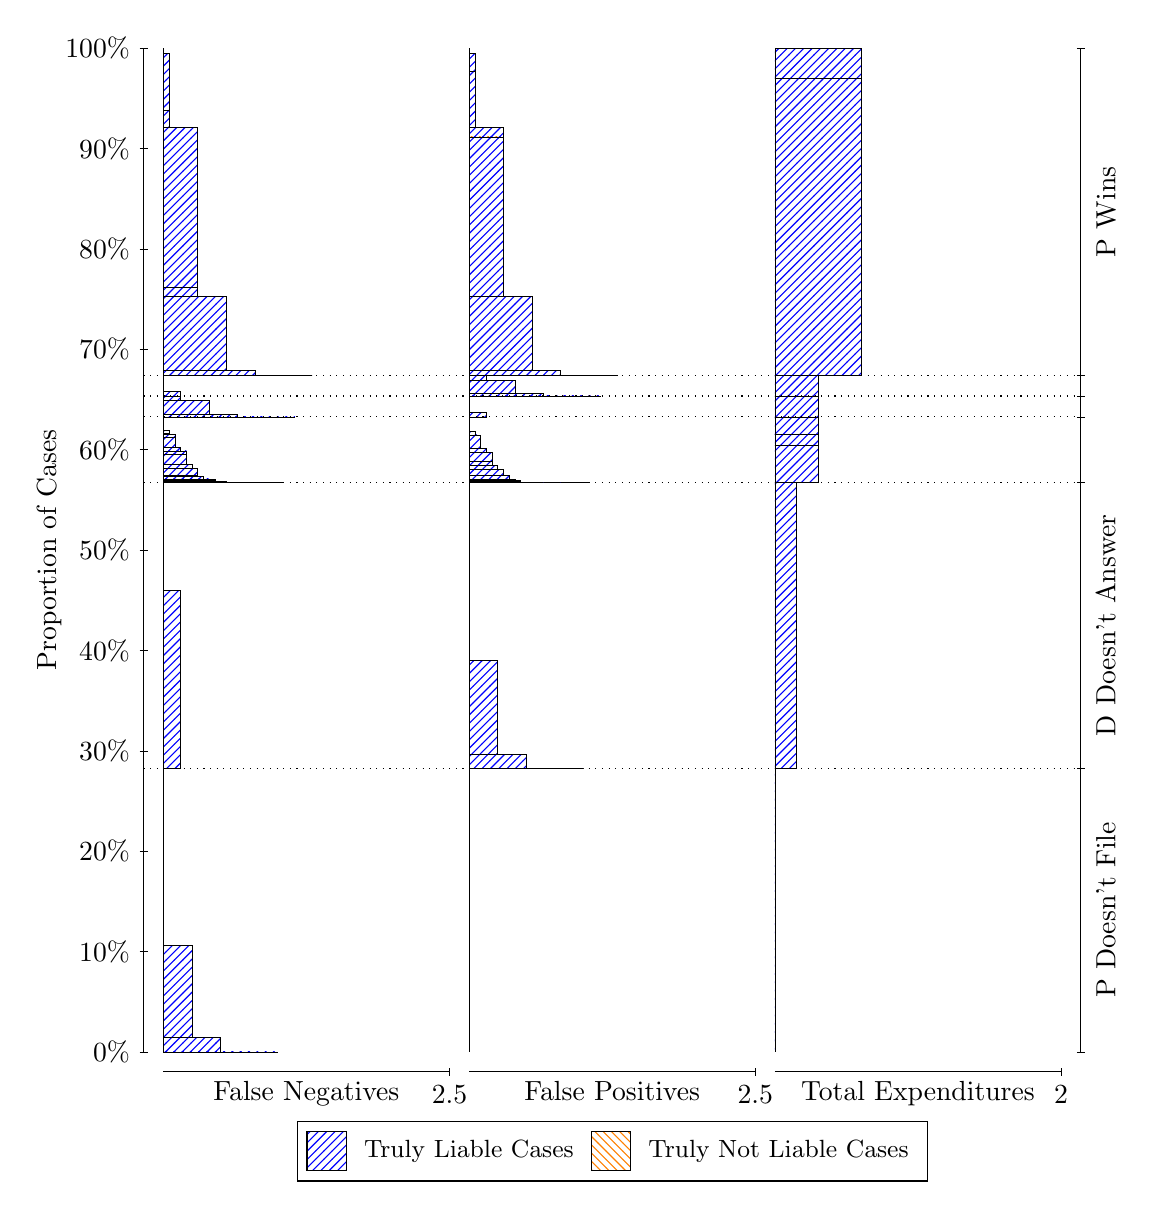
\begin{tikzpicture}
\draw[black, very thin] (1.5,1.75) -- (1.5,14.5);
\node[rotate=90, text=black, anchor=center] at (0.3, 8.125) {Proportion of Cases};
\draw[black, very thin] (1.45,1.75) -- (1.55,1.75);
\node[text=black, anchor=east] at (1.45, 1.75) {0\%};
\draw[black, very thin] (1.45,3.025) -- (1.55,3.025);
\node[text=black, anchor=east] at (1.45, 3.025) {10\%};
\draw[black, very thin] (1.45,4.3) -- (1.55,4.3);
\node[text=black, anchor=east] at (1.45, 4.3) {20\%};
\draw[black, very thin] (1.45,5.575) -- (1.55,5.575);
\node[text=black, anchor=east] at (1.45, 5.575) {30\%};
\draw[black, very thin] (1.45,6.85) -- (1.55,6.85);
\node[text=black, anchor=east] at (1.45, 6.85) {40\%};
\draw[black, very thin] (1.45,8.125) -- (1.55,8.125);
\node[text=black, anchor=east] at (1.45, 8.125) {50\%};
\draw[black, very thin] (1.45,9.4) -- (1.55,9.4);
\node[text=black, anchor=east] at (1.45, 9.4) {60\%};
\draw[black, very thin] (1.45,10.675) -- (1.55,10.675);
\node[text=black, anchor=east] at (1.45, 10.675) {70\%};
\draw[black, very thin] (1.45,11.95) -- (1.55,11.95);
\node[text=black, anchor=east] at (1.45, 11.95) {80\%};
\draw[black, very thin] (1.45,13.225) -- (1.55,13.225);
\node[text=black, anchor=east] at (1.45, 13.225) {90\%};
\draw[black, very thin] (1.45,14.5) -- (1.55,14.5);
\node[text=black, anchor=east] at (1.45, 14.5) {100\%};

\draw[black, very thin] (13.4,1.75) -- (13.4,14.5);
\draw[black, very thin] (13.35,1.75) -- (13.45,1.75);
\node[anchor=west] at (13.35, 1.75) {};
\draw[black, very thin] (13.35,5.3546) -- (13.45,5.3546);
\node[anchor=west] at (13.35, 5.3546) {};
\draw[black, very thin] (13.35,8.9808) -- (13.45,8.9808);
\node[anchor=west] at (13.35, 8.9808) {};
\draw[black, very thin] (13.35,9.8163) -- (13.45,9.8163);
\node[anchor=west] at (13.35, 9.8163) {};
\draw[black, very thin] (13.35,10.081) -- (13.45,10.081);
\node[anchor=west] at (13.35, 10.081) {};
\draw[black, very thin] (13.35,10.339) -- (13.45,10.339);
\node[anchor=west] at (13.35, 10.339) {};
\draw[black, very thin] (13.35,14.5) -- (13.45,14.5);
\node[anchor=west] at (13.35, 14.5) {};

\draw[black, very thin, pattern color=blue, pattern=north east lines] (1.75,1.75) rectangle (3.2033,1.75);
\draw[black, very thin, pattern color=blue, pattern=north east lines] (1.75,1.75) rectangle (2.84,1.7515);
\draw[black, very thin, pattern color=blue, pattern=north east lines] (1.75,1.7515) rectangle (2.4767,1.9339);
\draw[black, very thin, pattern color=blue, pattern=north east lines] (1.75,1.9339) rectangle (2.1133,3.1067);
\draw[black, very thin, pattern color=orange, pattern=north west lines] (1.75,3.1067) rectangle (1.75,3.1067);
\draw[black, very thin, pattern color=blue, pattern=north east lines] (1.75,3.1067) rectangle (1.75,5.3546);
\draw[black, very thin, pattern color=blue, pattern=north east lines] (1.75,5.3546) rectangle (1.968,7.6091);
\draw[black, very thin, pattern color=orange, pattern=north west lines] (1.75,7.6091) rectangle (1.75,7.6091);
\draw[black, very thin, pattern color=blue, pattern=north east lines] (1.75,7.6091) rectangle (1.75,8.9808);
\draw[black, very thin, pattern color=blue, pattern=north east lines] (1.75,8.9808) rectangle (3.276,8.9808);
\draw[black, very thin, pattern color=blue, pattern=north east lines] (1.75,8.9808) rectangle (3.1307,8.9808);
\draw[black, very thin, pattern color=blue, pattern=north east lines] (1.75,8.9808) rectangle (2.9853,8.9808);
\draw[black, very thin, pattern color=blue, pattern=north east lines] (1.75,8.9808) rectangle (2.9127,8.9808);
\draw[black, very thin, pattern color=blue, pattern=north east lines] (1.75,8.9808) rectangle (2.84,8.9808);
\draw[black, very thin, pattern color=blue, pattern=north east lines] (1.75,8.9808) rectangle (2.7673,8.9808);
\draw[black, very thin, pattern color=blue, pattern=north east lines] (1.75,8.9808) rectangle (2.6947,8.9809);
\draw[black, very thin, pattern color=blue, pattern=north east lines] (1.75,8.9809) rectangle (2.622,8.981);
\draw[black, very thin, pattern color=blue, pattern=north east lines] (1.75,8.981) rectangle (2.5493,8.9949);
\draw[black, very thin, pattern color=blue, pattern=north east lines] (1.75,8.9949) rectangle (2.4767,8.9951);
\draw[black, very thin, pattern color=blue, pattern=north east lines] (1.75,8.9951) rectangle (2.404,9.0111);
\draw[black, very thin, pattern color=blue, pattern=north east lines] (1.75,9.0111) rectangle (2.404,9.0195);
\draw[black, very thin, pattern color=blue, pattern=north east lines] (1.75,9.0195) rectangle (2.3313,9.0288);
\draw[black, very thin, pattern color=blue, pattern=north east lines] (1.75,9.0288) rectangle (2.2587,9.0646);
\draw[black, very thin, pattern color=blue, pattern=north east lines] (1.75,9.0646) rectangle (2.186,9.0763);
\draw[black, very thin, pattern color=blue, pattern=north east lines] (1.75,9.0763) rectangle (2.186,9.1634);
\draw[black, very thin, pattern color=blue, pattern=north east lines] (1.75,9.1634) rectangle (2.1133,9.2114);
\draw[black, very thin, pattern color=blue, pattern=north east lines] (1.75,9.2114) rectangle (2.0407,9.3464);
\draw[black, very thin, pattern color=blue, pattern=north east lines] (1.75,9.3464) rectangle (2.0407,9.3849);
\draw[black, very thin, pattern color=blue, pattern=north east lines] (1.75,9.3849) rectangle (1.968,9.4326);
\draw[black, very thin, pattern color=blue, pattern=north east lines] (1.75,9.4326) rectangle (1.8953,9.5513);
\draw[black, very thin, pattern color=blue, pattern=north east lines] (1.75,9.5513) rectangle (1.8953,9.5934);
\draw[black, very thin, pattern color=blue, pattern=north east lines] (1.75,9.5934) rectangle (1.8227,9.6074);
\draw[black, very thin, pattern color=blue, pattern=north east lines] (1.75,9.6074) rectangle (1.8227,9.6487);
\draw[black, very thin, pattern color=blue, pattern=north east lines] (1.75,9.6487) rectangle (1.75,9.6487);
\draw[black, very thin, pattern color=orange, pattern=north west lines] (1.75,9.6487) rectangle (1.75,9.6487);
\draw[black, very thin, pattern color=blue, pattern=north east lines] (1.75,9.6487) rectangle (1.75,9.8163);
\draw[black, very thin, pattern color=blue, pattern=north east lines] (1.75,9.8163) rectangle (3.4213,9.8163);
\draw[black, very thin, pattern color=blue, pattern=north east lines] (1.75,9.8163) rectangle (3.058,9.8164);
\draw[black, very thin, pattern color=blue, pattern=north east lines] (1.75,9.8164) rectangle (2.6947,9.8493);
\draw[black, very thin, pattern color=blue, pattern=north east lines] (1.75,9.8493) rectangle (2.3313,10.023);
\draw[black, very thin, pattern color=blue, pattern=north east lines] (1.75,10.023) rectangle (1.968,10.081);
\draw[black, very thin, pattern color=orange, pattern=north west lines] (1.75,10.081) rectangle (1.75,10.081);
\draw[black, very thin, pattern color=blue, pattern=north east lines] (1.75,10.081) rectangle (1.968,10.139);
\draw[black, very thin, pattern color=orange, pattern=north west lines] (1.75,10.139) rectangle (1.75,10.139);
\draw[black, very thin, pattern color=blue, pattern=north east lines] (1.75,10.139) rectangle (1.75,10.339);
\draw[black, very thin, pattern color=blue, pattern=north east lines] (1.75,10.339) rectangle (3.6393,10.339);
\draw[black, very thin, pattern color=blue, pattern=north east lines] (1.75,10.339) rectangle (3.276,10.34);
\draw[black, very thin, pattern color=blue, pattern=north east lines] (1.75,10.34) rectangle (2.9127,10.409);
\draw[black, very thin, pattern color=blue, pattern=north east lines] (1.75,10.409) rectangle (2.5493,11.348);
\draw[black, very thin, pattern color=blue, pattern=north east lines] (1.75,11.348) rectangle (2.186,11.465);
\draw[black, very thin, pattern color=blue, pattern=north east lines] (1.75,11.465) rectangle (2.186,13.49);
\draw[black, very thin, pattern color=blue, pattern=north east lines] (1.75,13.49) rectangle (1.8227,13.704);
\draw[black, very thin, pattern color=blue, pattern=north east lines] (1.75,13.704) rectangle (1.8227,14.429);
\draw[black, very thin, pattern color=orange, pattern=north west lines] (1.75,14.429) rectangle (1.75,14.429);
\draw[black, very thin, pattern color=blue, pattern=north east lines] (1.75,14.429) rectangle (1.75,14.5);
\draw[black, very thin, pattern color=orange, pattern=north west lines] (5.6333,1.75) rectangle (5.6333,1.75);
\draw[black, very thin, pattern color=blue, pattern=north east lines] (5.6333,1.75) rectangle (5.6333,5.3546);
\draw[black, very thin, pattern color=orange, pattern=north west lines] (5.6333,5.3546) rectangle (7.0867,5.3546);
\draw[black, very thin, pattern color=blue, pattern=north east lines] (5.6333,5.3546) rectangle (7.0867,5.3546);
\draw[black, very thin, pattern color=blue, pattern=north east lines] (5.6333,5.3546) rectangle (6.7233,5.3554);
\draw[black, very thin, pattern color=blue, pattern=north east lines] (5.6333,5.3554) rectangle (6.36,5.5299);
\draw[black, very thin, pattern color=blue, pattern=north east lines] (5.6333,5.5299) rectangle (5.9967,6.7263);
\draw[black, very thin, pattern color=blue, pattern=north east lines] (5.6333,6.7263) rectangle (5.6333,8.9808);
\draw[black, very thin, pattern color=orange, pattern=north west lines] (5.6333,8.9808) rectangle (7.1593,8.9808);
\draw[black, very thin, pattern color=blue, pattern=north east lines] (5.6333,8.9808) rectangle (7.1593,8.9808);
\draw[black, very thin, pattern color=orange, pattern=north west lines] (5.6333,8.9808) rectangle (7.014,8.9808);
\draw[black, very thin, pattern color=blue, pattern=north east lines] (5.6333,8.9808) rectangle (7.014,8.9808);
\draw[black, very thin, pattern color=orange, pattern=north west lines] (5.6333,8.9808) rectangle (6.8687,8.9808);
\draw[black, very thin, pattern color=blue, pattern=north east lines] (5.6333,8.9808) rectangle (6.8687,8.9808);
\draw[black, very thin, pattern color=blue, pattern=north east lines] (5.6333,8.9808) rectangle (6.796,8.9808);
\draw[black, very thin, pattern color=orange, pattern=north west lines] (5.6333,8.9808) rectangle (6.7233,8.9808);
\draw[black, very thin, pattern color=blue, pattern=north east lines] (5.6333,8.9808) rectangle (6.7233,8.9808);
\draw[black, very thin, pattern color=blue, pattern=north east lines] (5.6333,8.9808) rectangle (6.6507,8.9808);
\draw[black, very thin, pattern color=orange, pattern=north west lines] (5.6333,8.9808) rectangle (6.578,8.9808);
\draw[black, very thin, pattern color=blue, pattern=north east lines] (5.6333,8.9808) rectangle (6.578,8.9808);
\draw[black, very thin, pattern color=blue, pattern=north east lines] (5.6333,8.9808) rectangle (6.5053,8.981);
\draw[black, very thin, pattern color=orange, pattern=north west lines] (5.6333,8.981) rectangle (6.4327,8.981);
\draw[black, very thin, pattern color=blue, pattern=north east lines] (5.6333,8.981) rectangle (6.4327,8.9883);
\draw[black, very thin, pattern color=orange, pattern=north west lines] (5.6333,8.9883) rectangle (6.4327,8.9883);
\draw[black, very thin, pattern color=blue, pattern=north east lines] (5.6333,8.9883) rectangle (6.4327,8.9883);
\draw[black, very thin, pattern color=blue, pattern=north east lines] (5.6333,8.9883) rectangle (6.36,8.9884);
\draw[black, very thin, pattern color=blue, pattern=north east lines] (5.6333,8.9884) rectangle (6.2873,9.0001);
\draw[black, very thin, pattern color=orange, pattern=north west lines] (5.6333,9.0001) rectangle (6.2873,9.0001);
\draw[black, very thin, pattern color=blue, pattern=north east lines] (5.6333,9.0001) rectangle (6.2873,9.0157);
\draw[black, very thin, pattern color=blue, pattern=north east lines] (5.6333,9.0157) rectangle (6.2147,9.022);
\draw[black, very thin, pattern color=orange, pattern=north west lines] (5.6333,9.022) rectangle (6.142,9.022);
\draw[black, very thin, pattern color=blue, pattern=north east lines] (5.6333,9.022) rectangle (6.142,9.0701);
\draw[black, very thin, pattern color=blue, pattern=north east lines] (5.6333,9.0701) rectangle (6.0693,9.1483);
\draw[black, very thin, pattern color=blue, pattern=north east lines] (5.6333,9.1483) rectangle (6.0693,9.1484);
\draw[black, very thin, pattern color=orange, pattern=north west lines] (5.6333,9.1484) rectangle (5.9967,9.1484);
\draw[black, very thin, pattern color=blue, pattern=north east lines] (5.6333,9.1484) rectangle (5.9967,9.2037);
\draw[black, very thin, pattern color=blue, pattern=north east lines] (5.6333,9.2037) rectangle (5.924,9.2458);
\draw[black, very thin, pattern color=blue, pattern=north east lines] (5.6333,9.2458) rectangle (5.924,9.3644);
\draw[black, very thin, pattern color=blue, pattern=north east lines] (5.6333,9.3644) rectangle (5.8513,9.4122);
\draw[black, very thin, pattern color=blue, pattern=north east lines] (5.6333,9.4122) rectangle (5.7787,9.5857);
\draw[black, very thin, pattern color=blue, pattern=north east lines] (5.6333,9.5857) rectangle (5.706,9.6327);
\draw[black, very thin, pattern color=blue, pattern=north east lines] (5.6333,9.6327) rectangle (5.706,9.6336);
\draw[black, very thin, pattern color=blue, pattern=north east lines] (5.6333,9.6336) rectangle (5.6333,9.8163);
\draw[black, very thin, pattern color=orange, pattern=north west lines] (5.6333,9.8163) rectangle (5.8513,9.8163);
\draw[black, very thin, pattern color=blue, pattern=north east lines] (5.6333,9.8163) rectangle (5.8513,9.8742);
\draw[black, very thin, pattern color=blue, pattern=north east lines] (5.6333,9.8742) rectangle (5.6333,10.081);
\draw[black, very thin, pattern color=orange, pattern=north west lines] (5.6333,10.081) rectangle (7.3047,10.081);
\draw[black, very thin, pattern color=blue, pattern=north east lines] (5.6333,10.081) rectangle (7.3047,10.081);
\draw[black, very thin, pattern color=blue, pattern=north east lines] (5.6333,10.081) rectangle (6.9413,10.081);
\draw[black, very thin, pattern color=blue, pattern=north east lines] (5.6333,10.081) rectangle (6.578,10.111);
\draw[black, very thin, pattern color=blue, pattern=north east lines] (5.6333,10.111) rectangle (6.2147,10.281);
\draw[black, very thin, pattern color=blue, pattern=north east lines] (5.6333,10.281) rectangle (5.8513,10.339);
\draw[black, very thin, pattern color=orange, pattern=north west lines] (5.6333,10.339) rectangle (7.5227,10.339);
\draw[black, very thin, pattern color=blue, pattern=north east lines] (5.6333,10.339) rectangle (7.5227,10.339);
\draw[black, very thin, pattern color=orange, pattern=north west lines] (5.6333,10.339) rectangle (7.1593,10.339);
\draw[black, very thin, pattern color=blue, pattern=north east lines] (5.6333,10.339) rectangle (7.1593,10.34);
\draw[black, very thin, pattern color=orange, pattern=north west lines] (5.6333,10.34) rectangle (6.796,10.34);
\draw[black, very thin, pattern color=blue, pattern=north east lines] (5.6333,10.34) rectangle (6.796,10.41);
\draw[black, very thin, pattern color=orange, pattern=north west lines] (5.6333,10.41) rectangle (6.4327,10.41);
\draw[black, very thin, pattern color=blue, pattern=north east lines] (5.6333,10.41) rectangle (6.4327,11.35);
\draw[black, very thin, pattern color=blue, pattern=north east lines] (5.6333,11.35) rectangle (6.0693,13.372);
\draw[black, very thin, pattern color=orange, pattern=north west lines] (5.6333,13.372) rectangle (6.0693,13.372);
\draw[black, very thin, pattern color=blue, pattern=north east lines] (5.6333,13.372) rectangle (6.0693,13.491);
\draw[black, very thin, pattern color=blue, pattern=north east lines] (5.6333,13.491) rectangle (5.706,14.208);
\draw[black, very thin, pattern color=blue, pattern=north east lines] (5.6333,14.208) rectangle (5.706,14.43);
\draw[black, very thin, pattern color=blue, pattern=north east lines] (5.6333,14.43) rectangle (5.6333,14.5);
\draw[black, very thin, pattern color=orange, pattern=north west lines] (9.5167,1.75) rectangle (9.5167,1.75);
\draw[black, very thin, pattern color=blue, pattern=north east lines] (9.5167,1.75) rectangle (9.5167,5.3546);
\draw[black, very thin, pattern color=orange, pattern=north west lines] (9.5167,5.3546) rectangle (9.7892,5.3546);
\draw[black, very thin, pattern color=blue, pattern=north east lines] (9.5167,5.3546) rectangle (9.7892,8.9808);
\draw[black, very thin, pattern color=orange, pattern=north west lines] (9.5167,8.9808) rectangle (10.062,8.9808);
\draw[black, very thin, pattern color=blue, pattern=north east lines] (9.5167,8.9808) rectangle (10.062,9.4557);
\draw[black, very thin, pattern color=orange, pattern=north west lines] (9.5167,9.4557) rectangle (10.062,9.4557);
\draw[black, very thin, pattern color=blue, pattern=north east lines] (9.5167,9.4557) rectangle (10.062,9.598);
\draw[black, very thin, pattern color=orange, pattern=north west lines] (9.5167,9.598) rectangle (10.062,9.598);
\draw[black, very thin, pattern color=blue, pattern=north east lines] (9.5167,9.598) rectangle (10.062,9.8163);
\draw[black, very thin, pattern color=orange, pattern=north west lines] (9.5167,9.8163) rectangle (10.062,9.8163);
\draw[black, very thin, pattern color=blue, pattern=north east lines] (9.5167,9.8163) rectangle (10.062,10.081);
\draw[black, very thin, pattern color=orange, pattern=north west lines] (9.5167,10.081) rectangle (10.062,10.081);
\draw[black, very thin, pattern color=blue, pattern=north east lines] (9.5167,10.081) rectangle (10.062,10.339);
\draw[black, very thin, pattern color=orange, pattern=north west lines] (9.5167,10.339) rectangle (10.607,10.339);
\draw[black, very thin, pattern color=blue, pattern=north east lines] (9.5167,10.339) rectangle (10.607,14.115);
\draw[black, very thin, pattern color=orange, pattern=north west lines] (9.5167,14.115) rectangle (10.607,14.115);
\draw[black, very thin, pattern color=blue, pattern=north east lines] (9.5167,14.115) rectangle (10.607,14.5);
\draw[black, dotted] (1.5,5.3546) -- (13.4,5.3546);
\draw[black, dotted] (1.5,8.9808) -- (13.4,8.9808);
\draw[black, dotted] (1.5,9.8163) -- (13.4,9.8163);
\draw[black, dotted] (1.5,10.081) -- (13.4,10.081);
\draw[black, dotted] (1.5,10.339) -- (13.4,10.339);
\draw[black, very thin] (1.75,1.5) -- (5.3833,1.5);
\node[text=black, anchor=north] at (3.5667, 1.5) {False Negatives};
\draw[black, very thin] (5.3833,1.45) -- (5.3833,1.55);
\node[text=black, anchor=north] at (5.3833, 1.45) {2.5};

\draw[black, very thin] (5.6333,1.5) -- (9.2667,1.5);
\node[text=black, anchor=north] at (7.45, 1.5) {False Positives};
\draw[black, very thin] (9.2667,1.45) -- (9.2667,1.55);
\node[text=black, anchor=north] at (9.2667, 1.45) {2.5};

\draw[black, very thin] (9.5167,1.5) -- (13.15,1.5);
\node[text=black, anchor=north] at (11.333, 1.5) {Total Expenditures};
\draw[black, very thin] (13.15,1.45) -- (13.15,1.55);
\node[text=black, anchor=north] at (13.15, 1.45) {2};

\node[text=black, centered, rotate=90] at (13.72, 3.5523) {P Doesn't File};
\node[text=black, centered, rotate=90] at (13.72, 7.1677) {D Doesn't Answer};



\node[text=black, centered, rotate=90] at (13.72, 12.42) {P Wins};

\draw (7.449999999999999,1.5) node[draw=none] (baseCoordinate) {};
\begin{scope}[align=center]
        \matrix[scale=0.5, draw=black, below=0.5cm of baseCoordinate, nodes={draw}, column sep=0.1cm]{
            \node[rectangle, draw, minimum width=0.5cm, minimum height=0.5cm, pattern color=blue, pattern=north east lines] {}; &
            \node[draw=none, font=\small, text=black] (B) {Truly Liable Cases}; &
            \node[rectangle, draw, minimum width=0.5cm, minimum height=0.5cm, pattern color=orange, pattern=north west lines] {}; &
            \node[draw=none, font=\small, text=black] (B) {Truly Not Liable Cases}; \\
            };
\end{scope}

\end{tikzpicture}
\end{document}